%!TeX root=../tese.tex
%("dica" para o editor de texto: este arquivo é parte de um documento maior)
% para saber mais: https://tex.stackexchange.com/q/78101/183146

%% ------------------------------------------------------------------------- %%
\chapter{Introdução}
\label{cap:introducao}

\section{Motivação e Objetivos}

Com a crescente ascensão da tecnologia nos dias de hoje o conhecimento sobre
programação tem se tornado cada vez mais importante, não só pelas inúmeras
aplicações que existem, mas também por ser um facilitador, tanto na vida
pessoal quanto na vida profissional.

Devido a esse fato, houve um grande aumento no número de interessados pelo
conhecimento da programação e, consequentemente, o ensino de tal área tem se
difundido cada vez mais. Entretanto, muitos dos interessados por tais técnicas
não dispõem do tempo necessário ou da paciência e concentração para o 
aprendizado tradicional, ou seja, leituras extensas sobre os temas e longas 
sessões práticas para a aplicação das técnicas aprendidas.

Neste momento os jogos ganham força como disseminadores do conhecimento para os 
que buscam o primeiro contato com esta área, pois são
uma forma divertida e rápida de se adquirir experiência básica sobre algo.
Por ser uma forma simples e dinâmica de aprendizado o indíviduo encontra mais
facilidade para encaixar o jogo em sua agenda do que ler um livro teórico sobre
algo. Por isso que o jogo desenvolvido tenta \textit{gamificar} uma plataforma 
de ensino.

Desta forma, visando proporcionar um ambiente facilitador do aprendizado dos
conceitos de programação para indivíduos iniciantes ou com pouca experiência
foi desenvolvido o jogo Phoenix Rising. Além disso a estrutura do código foi
pensada de modo a facilitar a inserção de novas características ao jogo
pelos indivíduos que têm certa experiência em programação, fazendo com que
o projeto desenvolvido sirva para uma grande parte dos interessados em 
aprofundar o conhecimento.


%% ------------------------------------------------------------------------- %%
\section{Organização do Projeto}
\label{sec:consideracoes_preliminares}

O projeto foi desenvolvido utilizando Godot na versão 3.1.1 stable, 
uma \textit{game engine} que facilita a produção de jogos e possui uma linguagem
própria chamada GDScript.
Todo o código do jogo está mantido no GitHub, portanto o projeto é open source,
o que facilita a contribuição pela comunidade.

Como um dos objetivos do projeto é disponibilizar o código fonte para
melhorias serem implementadas, o código e comentários estão em inglês, seguindo
as boas práticas de programação. Vale salientar também que a eficiência não foi
principal ponto do projeto mas sim a legibilidade e a flexibilidade do 
código, portanto em algumas partes preferiu-se utilizar um pouco mais de memória
e/ou processamento, embora tais escolhas não tenham grande impacto na 
jogabilidade.

\section{Noção básica sobre o jogo}
\label{sec:consideracoes_preliminares}

Para conseguir completar o objetivo o jogo \textit{Phoenix Rising} funciona
da seguinte forma:

O jogador deve resolver o quebra cabeças conectando os blocos da forma correta
até que a Entrada esteja conectada com a Saída.

\begin{figure}[H]
    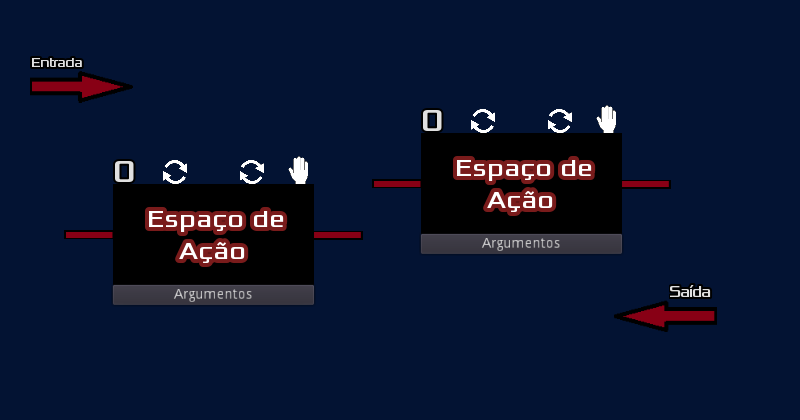
\includegraphics[width=\textwidth]{../figuras/jogo_nao_conectado.png}
    \caption{Jogo não conectado}
\end{figure}

\begin{figure}[H]
    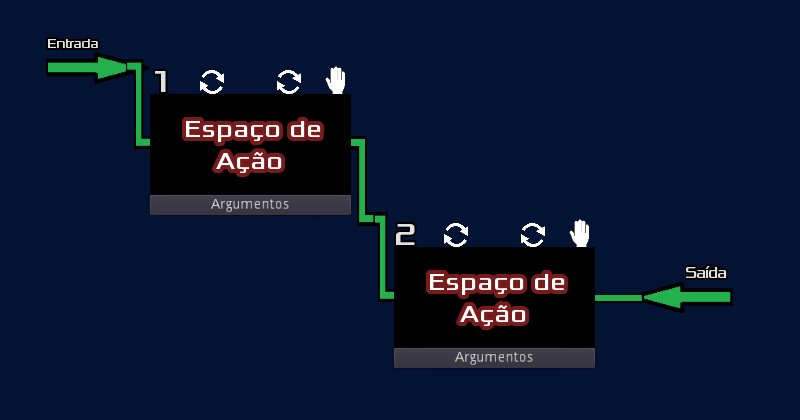
\includegraphics[width=\textwidth]{../figuras/jogo_conectado.png}
    \caption{Jogo conectado}
\end{figure}

Desta forma o jogador deve compreender que, para criar um programa, é necessário
pensar sobre a estrutura que o código terá antes de começar a utilizar os 
comandos, pois tentar criar um código apenas inserindo comandos sem pensar
previamente em uma estrutura base leva a códigos confusos e que muitas vezes
não funcionam corretamente. É claro que para sistemas maiores as reestruturações
do modelo ocorrem com certa frequência, porém o objetivo deste jogo é apenas
introduzir os conceitos básicos de programação.

Após ter o sistema conectado, o jogador deve utilizar os comandos que são
disponibilizados no inventário.

%\begin{figure}[H]
%    
\includegraphics[width=\textwidth]{../figuras/exemplo_comandos.png}
%    \caption{Exemplo de comandos disponíveis}
%\end{figure}

Depois de posicionar os comandos, o sistema estará pronto para ser executado.

%\begin{figure}[H]
%    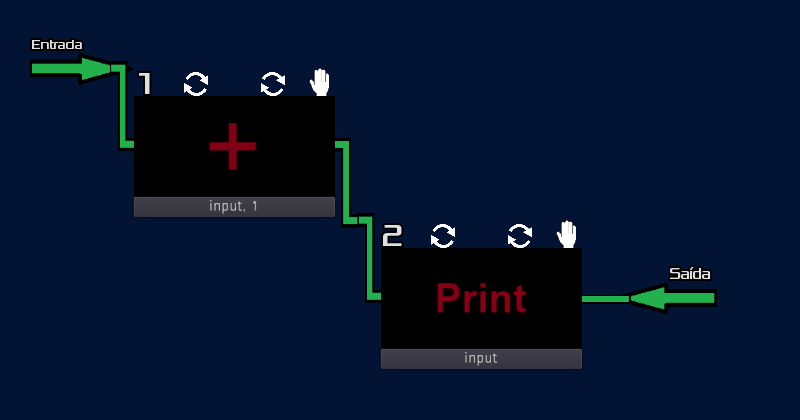
\includegraphics[width=\textwidth]{../figuras/sistema_pronto.png}
%    \caption{Sistema pronto para executar}
%\end{figure}

Para iniciar o processamento dos dados de entrada, ou seja, rodar o programa,
basta o jogador clicar no botão \textit{rodar!} e ficar atento à animação.

%\begin{figure}[H]
%    \includegraphics[width=\textwidth]{../figuras/inicio_da_execução.png}
%    \caption{Início da execução do sistema}
%\end{figure}